\documentclass[crop,tikz]{standalone}

\tikzset{>=latex}
\usetikzlibrary{decorations.markings}
\colorlet{gray}{gray!20}
\colorlet{green}{black!40!green}

\newcommand{\angl}{20}
\newcommand{\leng}{1.5}

\begin{document}
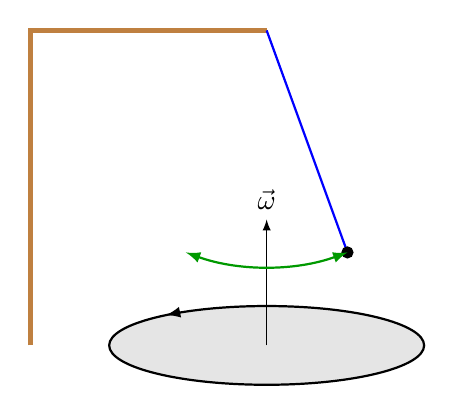
\begin{tikzpicture}[scale=2]
  \draw[thick,
        decoration={markings, mark=at position 0.4 with {\arrow{>}}},
        postaction={decorate},
        fill=gray
        ] (0,0) ellipse (1 and 0.25);
  \draw[->] (0,0) -- ++(0,0.8) node[above] {$\vec{\omega}$};
  \coordinate (a) at (0,2); % fixation
  \draw[line width=2pt,brown] (-1.5,0) -- ++ (0,2) -- (a);
  \draw[blue,thick] (a) -- ++(-90+\angl:\leng) coordinate (m);
  \draw[fill] (m) circle (1pt);
  \draw[<->,green,thick] (m) arc (-90+\angl:-90-\angl:\leng);
\end{tikzpicture}
\end{document}
